\clearpage

\refstepcounter{chapter}
\chapter*{Implementación}

\addcontentsline{toc}{chapter}{\protect\numberline{\thechapter}Implementación}
\vspace{-1.5cm} 
\noindent\HRule\par\vspace{0.1cm}

\section{Solución Software}




\subsection{Arquitectura del Sistema}

La arquitectura del sistema se plantea como un lazo cerrado de seguimiento visual, donde la información captada por la cámara se transforma progresivamente en órdenes de control para el UAV cazador. La Figura \ref{fig:arquitectura_nodos} resume este flujo completo, desde la adquisición de la imagen hasta el envío de consignas al autopiloto mediante \textit{MAVROS}.



\vspace{0.2cm}



\begin{figure}[H]
    \centering
    \resizebox{\textwidth}{!}{%
    \begin{tikzpicture}[
        node distance=1.8cm and 1.9cm,
        block/.style={rectangle, draw, fill=blue!10, text width=2.8cm, align=center, rounded corners, minimum height=1.1cm, font=\sffamily\small},
        pid/.style={rectangle, draw, fill=green!10, text width=3.2cm, align=center, rounded corners, minimum height=1.2cm, font=\sffamily\small},
        command/.style={rectangle, draw, fill=orange!15, text width=3.2cm, align=center, rounded corners, minimum height=1.2cm, font=\sffamily\small},
        arrow/.style={-{Latex[length=3mm]}, thick},
        feedback/.style={-{Latex[length=3mm]}, thick, dashed},
        flowlabel/.style={font=\footnotesize, fill=white, inner sep=1.5pt, align=center}
    ]

    \node [block] (cam) at (0, -2.6) {Cámara\\real o simulada};
    \node [block] (yolo) at (0, 2.4) {YOLOv8n};
    \node [block] (filtro) at (9.4, 2.4) {Kalman + EMA};
    \node [block] (errores) at (9.4, 0.0) {Cálculo de errores};

    \node [pid] (pidyaw) at (4.7, -2.6) {PID de \textit{yaw}};
    \node [pid] (pidz) at (9.4, -2.6) {PID de altura};
    \node [pid] (piddist) at (14.1, -2.6) {PID de distancia};
    \node [block] (mavros) at (9.4, -5.0) {MAVROS /\\controlador de vuelo};
    \node [block] (uav) at (9.4, -7.4) {UAV real o\\Gazebo/SITL};

    \draw [arrow] (cam) -- node[right, font=\footnotesize] {Imágenes RGB} (yolo);
    \draw [arrow] (yolo) -- node[above, flowlabel] {caja YOLO\\$(x_1,y_1,x_2,y_2)$} (filtro);
    \draw [arrow] (filtro.south) -- node[right, flowlabel] {caja suavizada\\centro, ancho, alto} (errores.north);

    \draw [arrow] (errores.south west) -- node[above, sloped, flowlabel] {\texttt{ex\_virtual}} (pidyaw.north east);
    \draw [arrow] (errores.south) -- node[right, flowlabel] {\texttt{ey\_virtual}} (pidz.north);
    \draw [arrow] (errores.south east) -- node[above, sloped, flowlabel] {\texttt{e\_dist}} (piddist.north west);

    \draw [arrow] (pidyaw.south east) -- node[below, sloped, flowlabel] {\texttt{w\_yaw}} (mavros.north west);
    \draw [arrow] (pidz.south) -- node[right, flowlabel] {\texttt{v\_y}} (mavros.north);
    \draw [arrow] (piddist.south west) -- node[below, sloped, flowlabel] {\texttt{v\_x}} (mavros.north east);

    \draw [arrow] (mavros) -- node[right, flowlabel] {MAVLink / setpoints} (uav);
    \draw [feedback] (uav.west) -| node[pos=0.25, below, flowlabel] {movimiento\\nueva imagen} (cam.south);

    \end{tikzpicture}%
    }
    \caption{Arquitectura general del sistema de seguimiento visual, válida tanto para simulación como para despliegue real. Elaboración propia.}
    \label{fig:arquitectura_nodos}
\end{figure}

Como se observa en la Figura \ref{fig:arquitectura_nodos}, el proceso comienza en la cámara real o simulada, que proporciona imágenes RGB del entorno. Estas imágenes son procesadas por YOLOv8n, que detecta el UAV objetivo y genera la caja delimitadora de la detección mediante las coordenadas $(x_1,y_1,x_2,y_2)$. Esta información constituye la entrada del bloque de filtrado, donde se aplica Kalman + EMA para suavizar las variaciones entre fotogramas y obtener una caja más estable.

\vspace{0.3cm}

A partir de la caja suavizada se calcula el centro aparente del objetivo, su anchura y su altura. Con estos datos se obtienen los tres errores que alimentan el control: \texttt{ex\_virtual}, asociado al desplazamiento horizontal; \texttt{ey\_virtual}, asociado al desplazamiento vertical; y \texttt{e\_dist}, asociado a la diferencia entre la distancia estimada y la distancia deseada de seguimiento.

\vspace{0.3cm}

Cada uno de estos errores se envía a un PID independiente. El PID de \textit{yaw} genera la velocidad angular \texttt{w\_yaw}, el PID de altura genera la velocidad vertical \texttt{v\_y} y el PID de distancia genera la velocidad frontal \texttt{v\_x}. Las tres salidas llegan al bloque \textit{MAVROS} / controlador de vuelo, que las convierte en consignas compatibles con el autopiloto. Finalmente, el movimiento del UAV modifica de nuevo la imagen recibida por la cámara, cerrando el lazo de realimentación visual del sistema.

\subsection{Nodos y Scripts Desarrollados}

En esta sección se describe la arquitectura de nodos y tópicos utilizados para integrar la percepción visual, la estimación del error y el control del UAV cazador. También se resumen los tópicos ROS más importantes observados mediante \texttt{rostopic list}, diferenciando entre los tópicos propios del sistema y los generados automáticamente por \textit{Gazebo}, \textit{MAVROS} y los sensores simulados.

\vspace{0.3cm}

Para visualizar la evolución de la arquitectura se emplea \texttt{rqt\_graph}, que permite observar de forma gráfica qué nodos están activos y cómo se comunican mediante tópicos. En primer lugar, se muestra el sistema justo después de iniciar la simulación, sin activar todavía los nodos de visión ni el nodo de control. En esta etapa aparecen principalmente los nodos y conexiones asociados a \textit{Gazebo}, \textit{MAVROS}, la cámara simulada y los tópicos de soporte de ROS.

\begin{center}
\refstepcounter{figure}\label{fig:rqt-graph-primero}
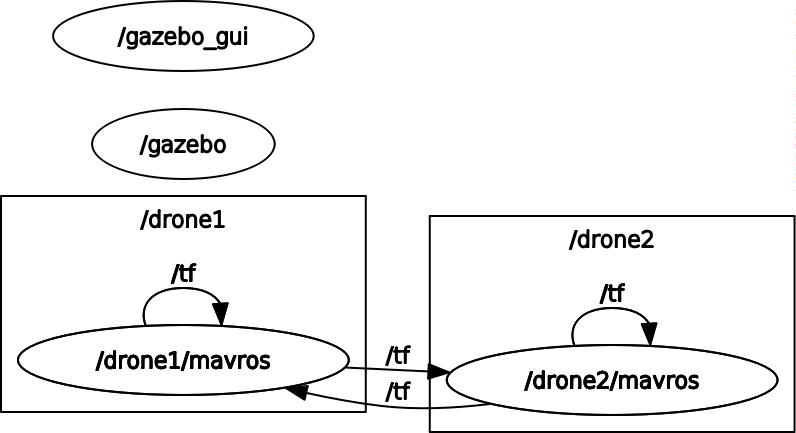
\includegraphics[width=0.95\textwidth]{imagenes/rosgraph_primero.png}\\[0.5ex]
{\small \textbf{Figura \thefigure.} Grafo inicial del sistema sin nodos de visión ni control activos. Imagen de elaboración propia.}
\addcontentsline{lof}{figure}{\protect\numberline{\thefigure}Grafo inicial del sistema sin nodos de visión ni control activos}
\end{center}

\vspace{0.3cm}

Posteriormente se activan los nodos de visión. En este segundo estado aparecen el nodo \texttt{yolo\_sender\_node}, encargado de procesar la imagen y publicar las coordenadas de la caja detectada, y el nodo \texttt{drone\_projection\_opencv\_node}, encargado de recibir la detección, calcular el centro visual, aplicar la compensación de actitud y publicar el error visual. En el grafo se observa cómo la imagen de la cámara alimenta al nodo de YOLO y cómo sus salidas se conectan con el nodo de proyección.

\begin{center}
\refstepcounter{figure}\label{fig:rqt-graph-segundo}
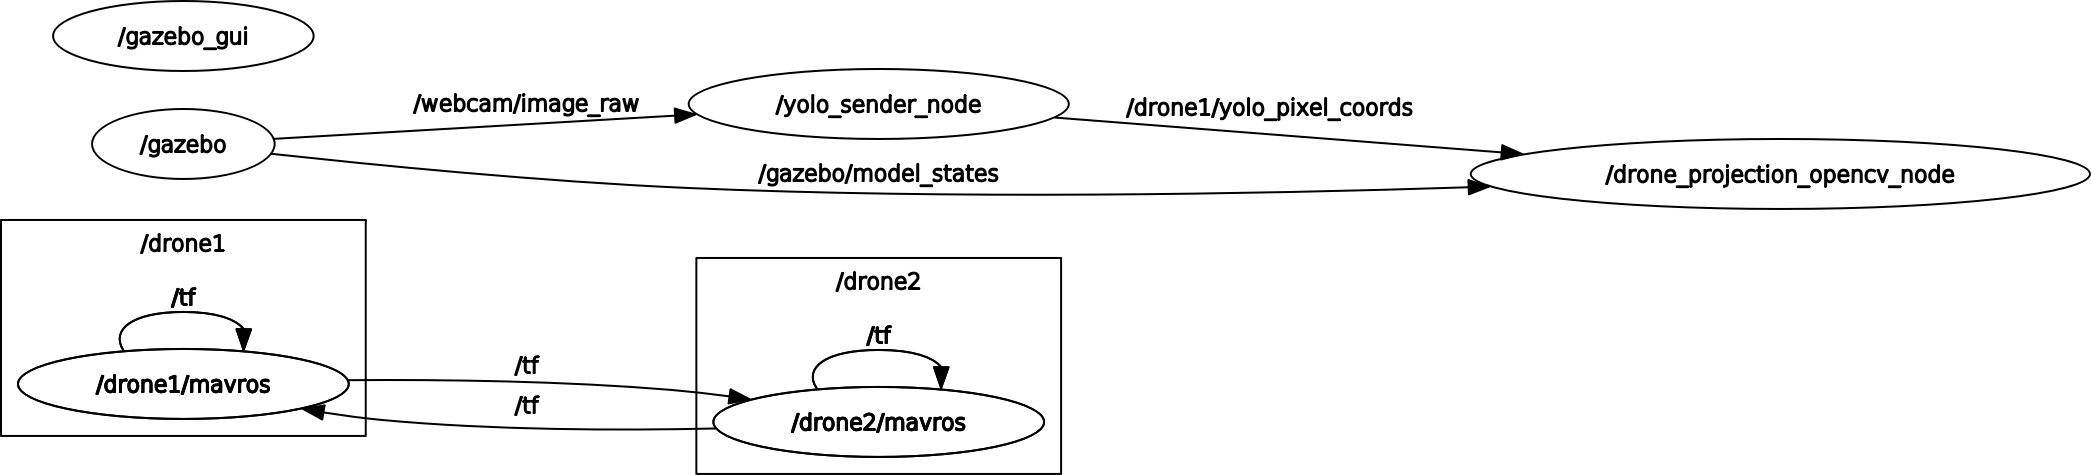
\includegraphics[width=1.0\textwidth]{imagenes/rosgraph_segundo.png}\\[0.5ex]
{\small \textbf{Figura \thefigure.} Grafo del sistema con los nodos de visión activados. Imagen de elaboración propia.}
\addcontentsline{lof}{figure}{\protect\numberline{\thefigure}Grafo del sistema con los nodos de visión activados}
\end{center}

\vspace{0.3cm}

Finalmente, se activa el nodo de control \texttt{drone1\_follow\_xy\_pid}. Este nodo recibe el error publicado por \texttt{drone\_projection\_opencv\_node} a través de \verb|/drone1/vision_error|, comprueba el estado del UAV mediante \verb|/drone1/mavros/state| y publica las consignas de velocidad en \verb|/drone1/mavros/setpoint_velocity/cmd_vel|. Con ello queda cerrado el flujo completo entre percepción, estimación del error, control y autopiloto.

\begin{center}
\refstepcounter{figure}\label{fig:rqt-graph-tercero}
\rotatebox{90}{%
\begin{minipage}{0.98\textheight}
\centering
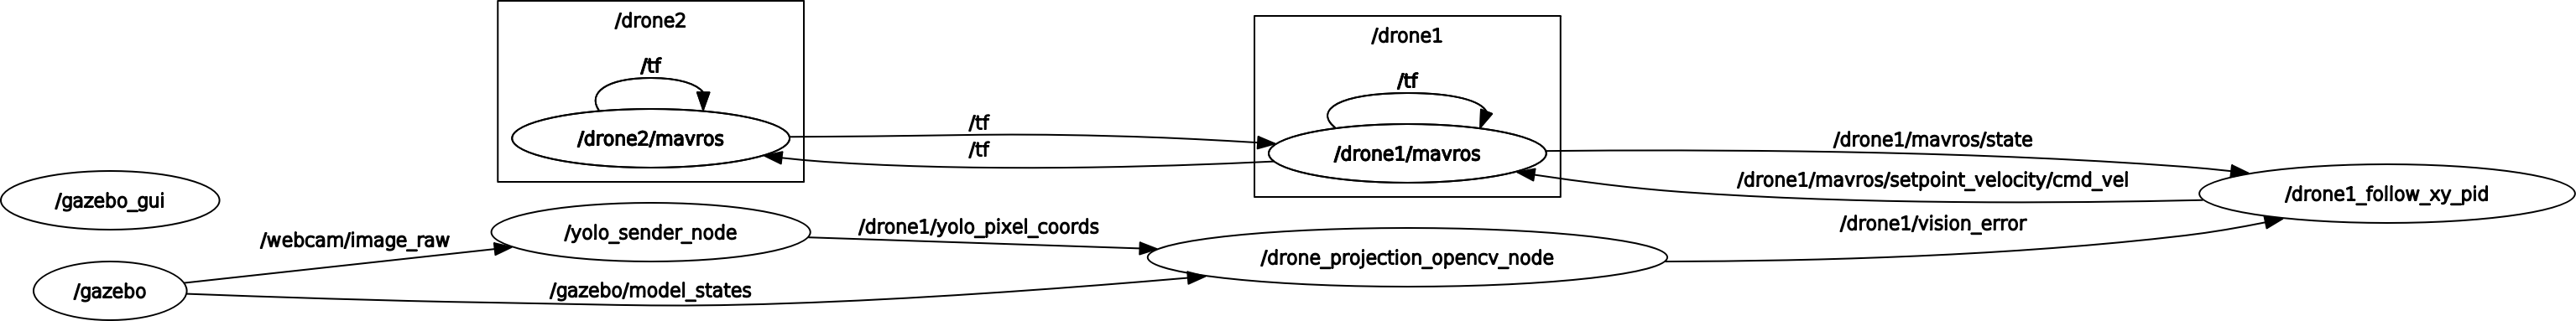
\includegraphics[width=1.0\textheight]{imagenes/rosgraph_tercero.png}\\[0.8ex]
{\small \textbf{Figura \thefigure.} Grafo completo del sistema con visión y control activos. Imagen de elaboración propia.}
\end{minipage}%
}
\addcontentsline{lof}{figure}{\protect\numberline{\thefigure}Grafo completo del sistema con visión y control activos}
\end{center}

\vspace{0.3cm}

\begin{center}
\refstepcounter{figure}\label{fig:topic-list}
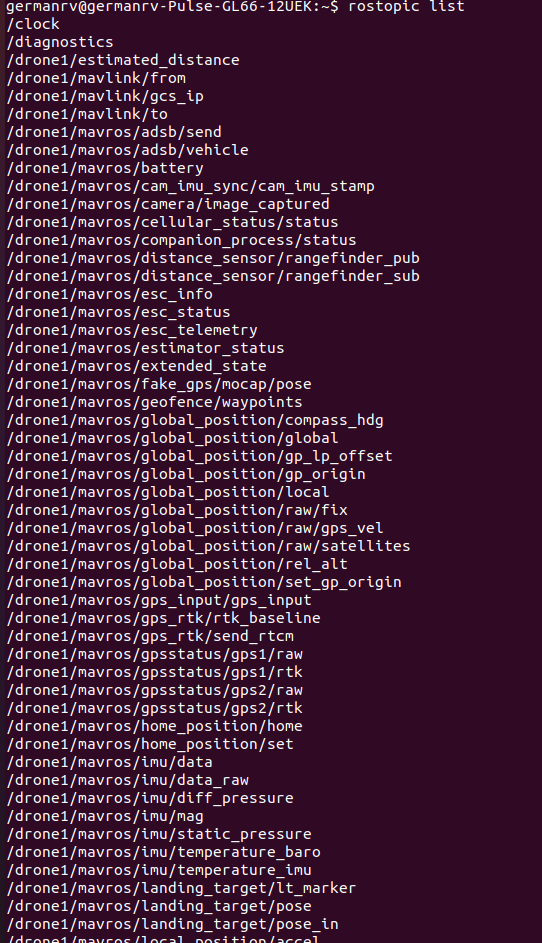
\includegraphics[width=0.75\textwidth]{imagenes/TopicList.png}\\[0.5ex]
{\small \textbf{Figura \thefigure.} Listado de  algunos tópicos ROS obtenido mediante \texttt{rostopic list}. Imagen de elaboración propia.}
\addcontentsline{lof}{figure}{\protect\numberline{\thefigure}Listado de tópicos ROS obtenido mediante rostopic list}
\end{center}

\vspace{0.3cm}

La salida de \texttt{rostopic list} muestra una gran cantidad de tópicos porque se lanzan dos instancias de UAV, cada una con su propio espacio de nombres de \textit{MAVROS}. Sin embargo, para el funcionamiento del sistema propuesto, los tópicos más relevantes son los siguientes:

\begin{itemize}
    \item \verb|/webcam/image_raw|: imagen RGB de entrada utilizada por YOLO y por el nodo de proyección para visualizar la detección y calcular el error sobre el plano de imagen.
    \item \verb|/webcam/camera_info|: información de calibración de la cámara. Aunque en la implementación también se cargan parámetros desde archivo, este tópico representa la fuente estándar de parámetros intrínsecos en ROS.
    \item \verb|/drone1/yolo_pixel_coords|: tópico publicado por el nodo de YOLO con las cuatro coordenadas de la caja delimitadora del objetivo, codificadas como \texttt{Quaternion}: $x_1$, $y_1$, $x_2$ e $y_2$.
    \item \verb|/drone1/yolo_state|: tópico de estado de la detección. El valor 0 indica objetivo perdido, el valor 1 indica detección directa de YOLO y el valor 2 indica predicción temporal mediante Kalman.

    \item \verb|/drone1/vision_error|: tópico publicado por el nodo de proyección. Contiene el error horizontal, el error vertical y el error de distancia en un mensaje \texttt{PointStamped}, que posteriormente consume el controlador PID.
    \item \verb|/drone1/mavros/state|: estado de conexión, armado y modo de vuelo del UAV cazador. El controlador lo consulta antes de publicar órdenes para evitar actuar cuando el dron no está listo.
    \item \verb|/drone1/mavros/setpoint_velocity/cmd_vel|: tópico de salida del controlador. En él se publican las velocidades lineales y angulares que \textit{MAVROS} envía al autopiloto para mover el dron cazador.
    \item \verb|/gazebo/model_states|: poses de los modelos simulados en \textit{Gazebo}. Se utiliza para obtener la pose de \texttt{drone1} y \texttt{drone2}, comprobar la geometría de la simulación y apoyar la compensación/proyección.
    
\end{itemize}

\vspace{0.3cm}

De forma resumida, el flujo de información comienza en \verb|/webcam/image_raw|, pasa por el nodo YOLO, se transforma en coordenadas de caja mediante \verb|/drone1/yolo_pixel_coords|, se convierte en error visual y longitudinal en \verb|/drone1/vision_error| y finalmente se traduce en comandos de velocidad publicados en \verb|/drone1/mavros/setpoint_velocity/cmd_vel|. El resto de tópicos de \textit{MAVROS} que aparecen bajo \verb|/drone1/mavros/| y \verb|/drone2/mavros/| corresponden a telemetría, sensores, misiones, parámetros y servicios auxiliares generados automáticamente por la interfaz con el autopiloto.

\section{Componente de Percepción}

\subsection{Entrenamiento de Modelos YOLO}

El modelo de detección finalmente integrado en el sistema fue YOLOv8n. Esta arquitectura se seleccionó mediante un torneo comparativo entre distintas variantes de YOLO, atendiendo al equilibrio entre precisión, tiempo de inferencia y tamaño del modelo. Dicho proceso de selección se detalla en la sección de experimentación, mientras que en este apartado se describe la preparación del conjunto de datos y el entrenamiento del modelo elegido.

\vspace{0.3cm}

Antes del entrenamiento se aplicó un preprocesamiento común a todas las imágenes del dataset. En primer lugar, todas las muestras se redimensionaron a $640 \times 640$ píxeles mediante un ajuste de tipo \textit{Fit}, manteniendo la relación de aspecto original e incorporando bordes negros cuando fue necesario. Este formato coincide con el tamaño de entrada empleado durante el entrenamiento de YOLOv8n y permite trabajar con imágenes homogéneas sin deformar el objeto de interés.

\vspace{0.3cm}

Sobre el dataset preprocesado se aplicó un proceso de aumento de datos con el objetivo de mejorar la capacidad de generalización del detector. Las transformaciones utilizadas fueron volteo horizontal, recorte con zoom mínimo del 0\% y zoom máximo del 13\%, variación de saturación entre $-4\%$ y $+4\%$, y variación de exposición entre $-8\%$ y $+8\%$. Estas modificaciones permiten que el modelo observe el UAV objetivo en condiciones visuales ligeramente distintas, simulando cambios de posición, escala, iluminación y color. De esta forma se reduce la dependencia respecto a las imágenes originales y se aumenta la robustez frente a situaciones que pueden aparecer durante la simulación o en un despliegue real.

\vspace{0.3cm}

Tras aplicar el preprocesamiento y el aumento de datos, el conjunto final quedó formado por 9651 imágenes. La división empleada para el entrenamiento fue de 6755 imágenes para \textit{train}, 1447 imágenes para \textit{valid} y 1449 imágenes para \textit{test}. Esta separación permitió entrenar el modelo con la mayor parte de los datos, supervisar su evolución sobre un conjunto de validación independiente y reservar un subconjunto final para comprobar posteriormente el comportamiento del detector.

\vspace{0.3cm}

El entrenamiento se realizó en Google Colab, donde se cargó el dataset ya organizado y se configuró el archivo YAML correspondiente con las rutas de entrenamiento, validación y prueba. Como YOLOv8n ya dispone de pesos preentrenados, el proceso se planteó como un ajuste fino sobre el modelo base \texttt{yolov8n.pt}, en lugar de entrenar la red desde cero. La ejecución se configuró para entrenar durante 30 épocas, con imágenes de entrada de $640 \times 640$ píxeles y un tamaño de lote de 16. Además, se activó la generación de gráficas del entrenamiento para analizar posteriormente la evolución de las pérdidas, las métricas de validación y los ejemplos de detección obtenidos.

\vspace{0.3cm}

Se mantuvieron los parámetros por defecto proporcionados por Ultralytics para el entrenamiento, dejando que la opción \texttt{optimizer=auto} seleccionara automáticamente el optimizador y los hiperparámetros principales. En este caso, el entrenamiento utilizó AdamW con \texttt{lr=0.002} y \texttt{momentum=0.9}, con pesos preentrenados activados mediante \texttt{pretrained=True}. Esto permitió aprovechar las características visuales ya aprendidas por YOLOv8n y adaptar únicamente el detector al UAV objetivo del dataset generado.

\vspace{0.3cm}

La evolución del entrenamiento se resume en la Figura \ref{fig:yolo-training-results}. En ella se observa que las pérdidas asociadas a la localización de la caja, la clasificación y la función DFL disminuyen de forma progresiva tanto en entrenamiento como en validación. Al mismo tiempo, las métricas de precisión, \textit{recall}, \textit{mAP50} y \textit{mAP50-95} aumentan y se estabilizan en valores elevados, lo que indica que el modelo aprende a detectar el UAV objetivo sin mostrar una divergencia clara entre entrenamiento y validación.

\begin{figure}[H]
\centering
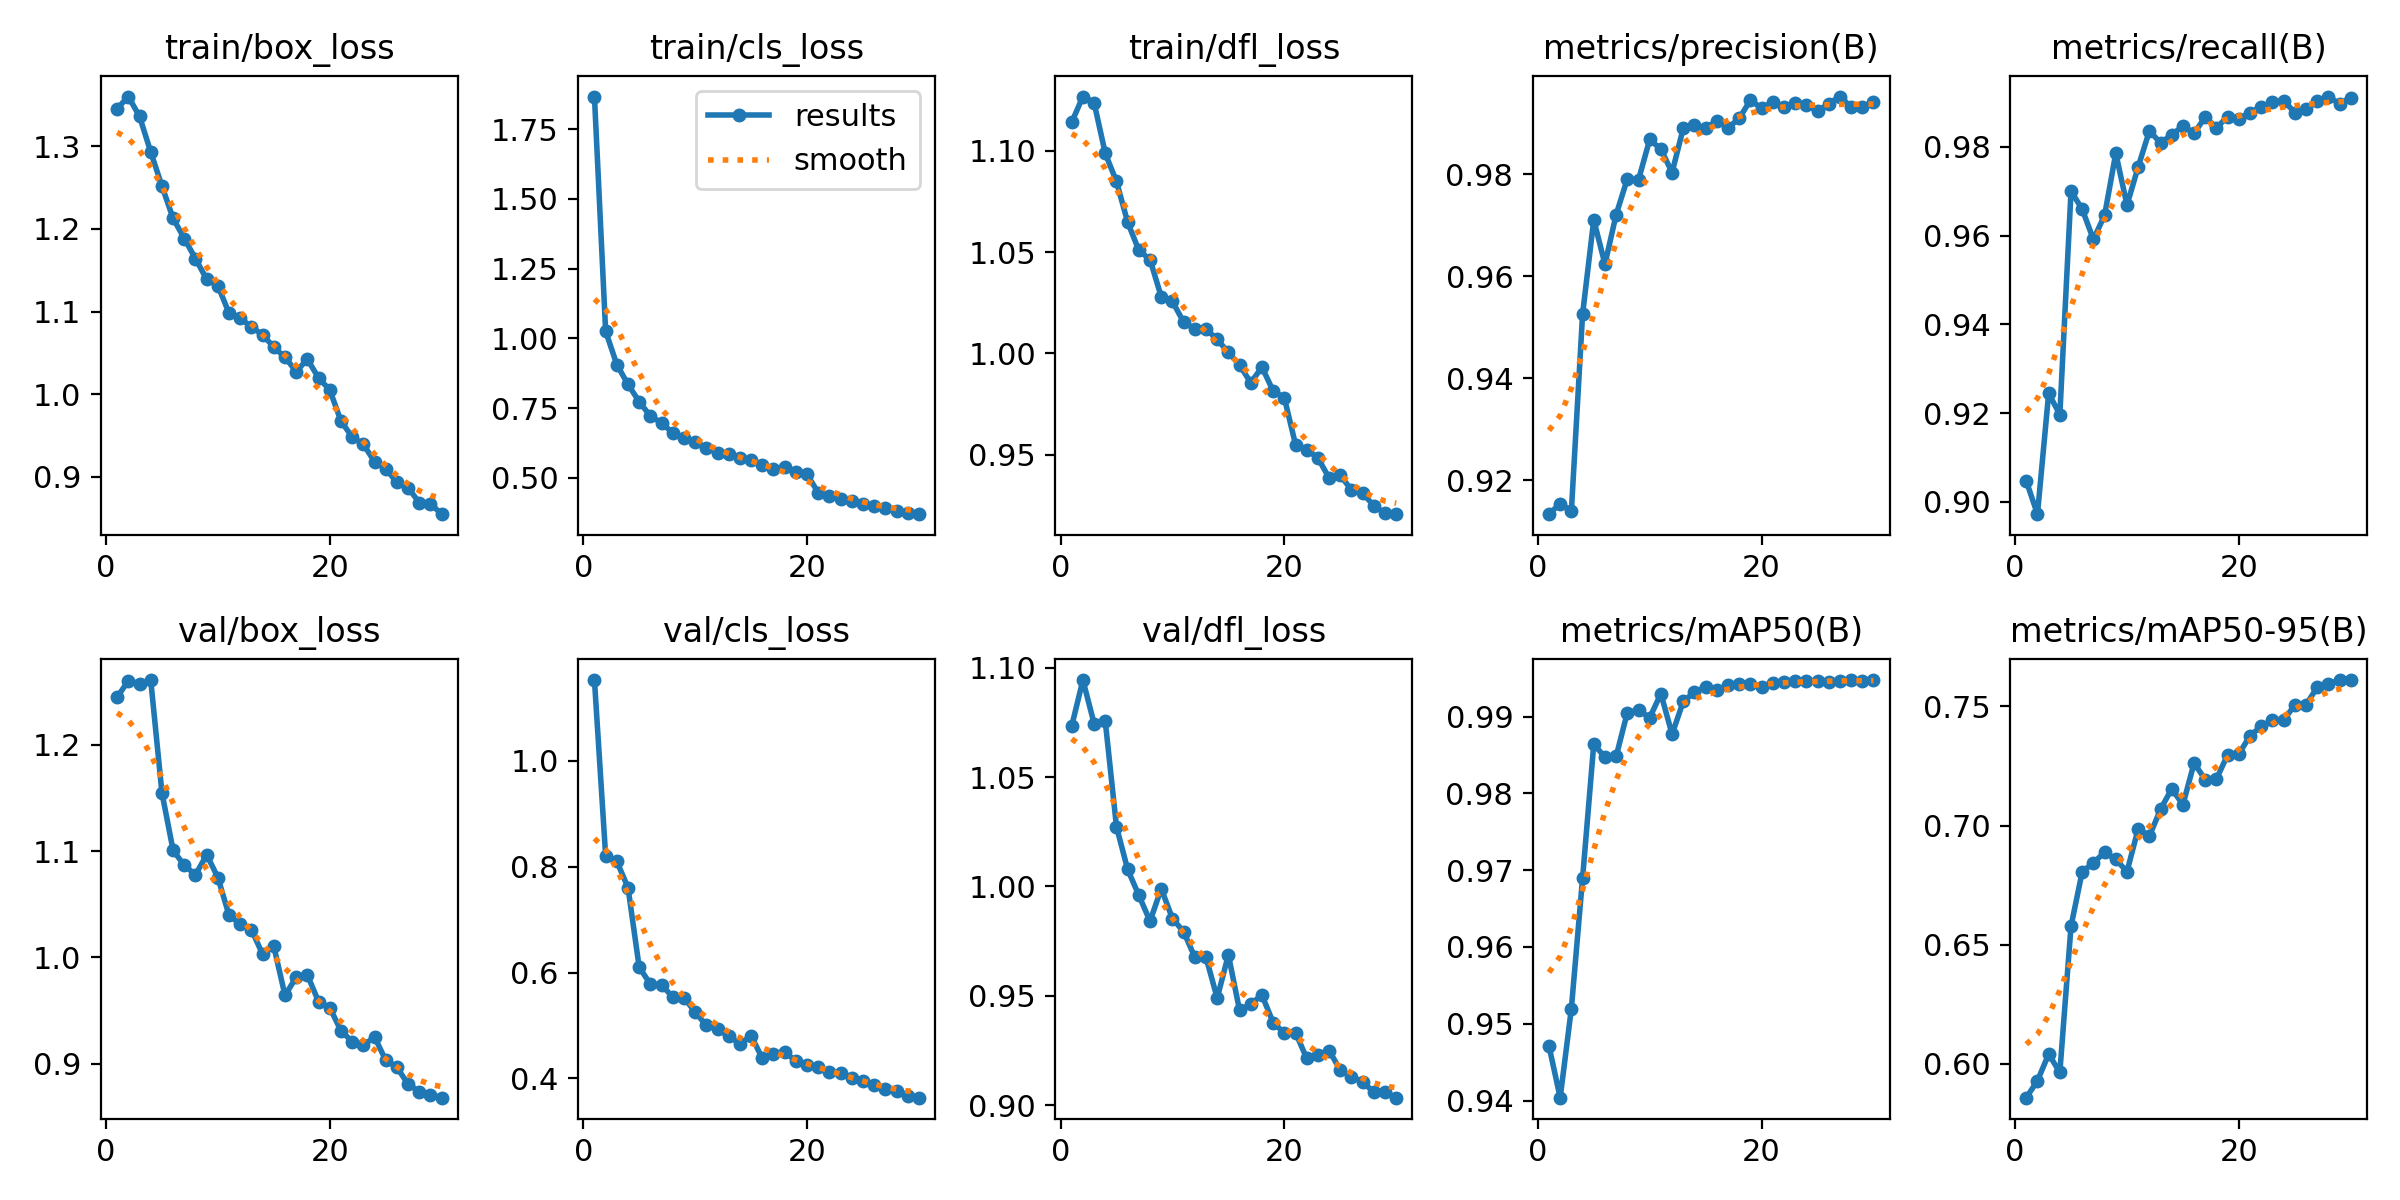
\includegraphics[width=1.0\textwidth]{imagenes/results.png}
\caption{Evolución de pérdidas y métricas durante el entrenamiento de YOLOv8n. Imagen de elaboración propia.}
\label{fig:yolo-training-results}
\end{figure}

\vspace{0.3cm}

La evolución de las últimas épocas confirma esta convergencia estable. En la época 18 se obtuvo una precisión de 0.992, un \textit{recall} de 0.991, un \textit{mAP50} de 0.995 y un \textit{mAP50-95} de 0.745. En la época 19 el \textit{mAP50-95} aumentó hasta 0.753, mientras que en la época 20 alcanzó 0.755, con una precisión de 0.996, un \textit{recall} de 0.994 y un \textit{mAP50} de 0.995. Al mismo tiempo, las pérdidas de entrenamiento continuaron descendiendo: la pérdida de caja pasó de 0.9271 a 0.8929, la pérdida de clasificación de 0.4212 a 0.3953 y la pérdida DFL de 0.9452 a 0.9339 entre las épocas 18 y 20.

\vspace{0.3cm}

La matriz de confusión de la Figura \ref{fig:yolo-confusion-matrix} refuerza esta conclusión, ya que concentra la mayor parte de las predicciones en la clase correcta y muestra una separación clara entre el UAV objetivo y el fondo. Este resultado es especialmente importante para el sistema de seguimiento, porque una confusión frecuente con el fondo provocaría cajas falsas, errores visuales incorrectos y órdenes de control innecesarias.

\begin{figure}[H]
\centering
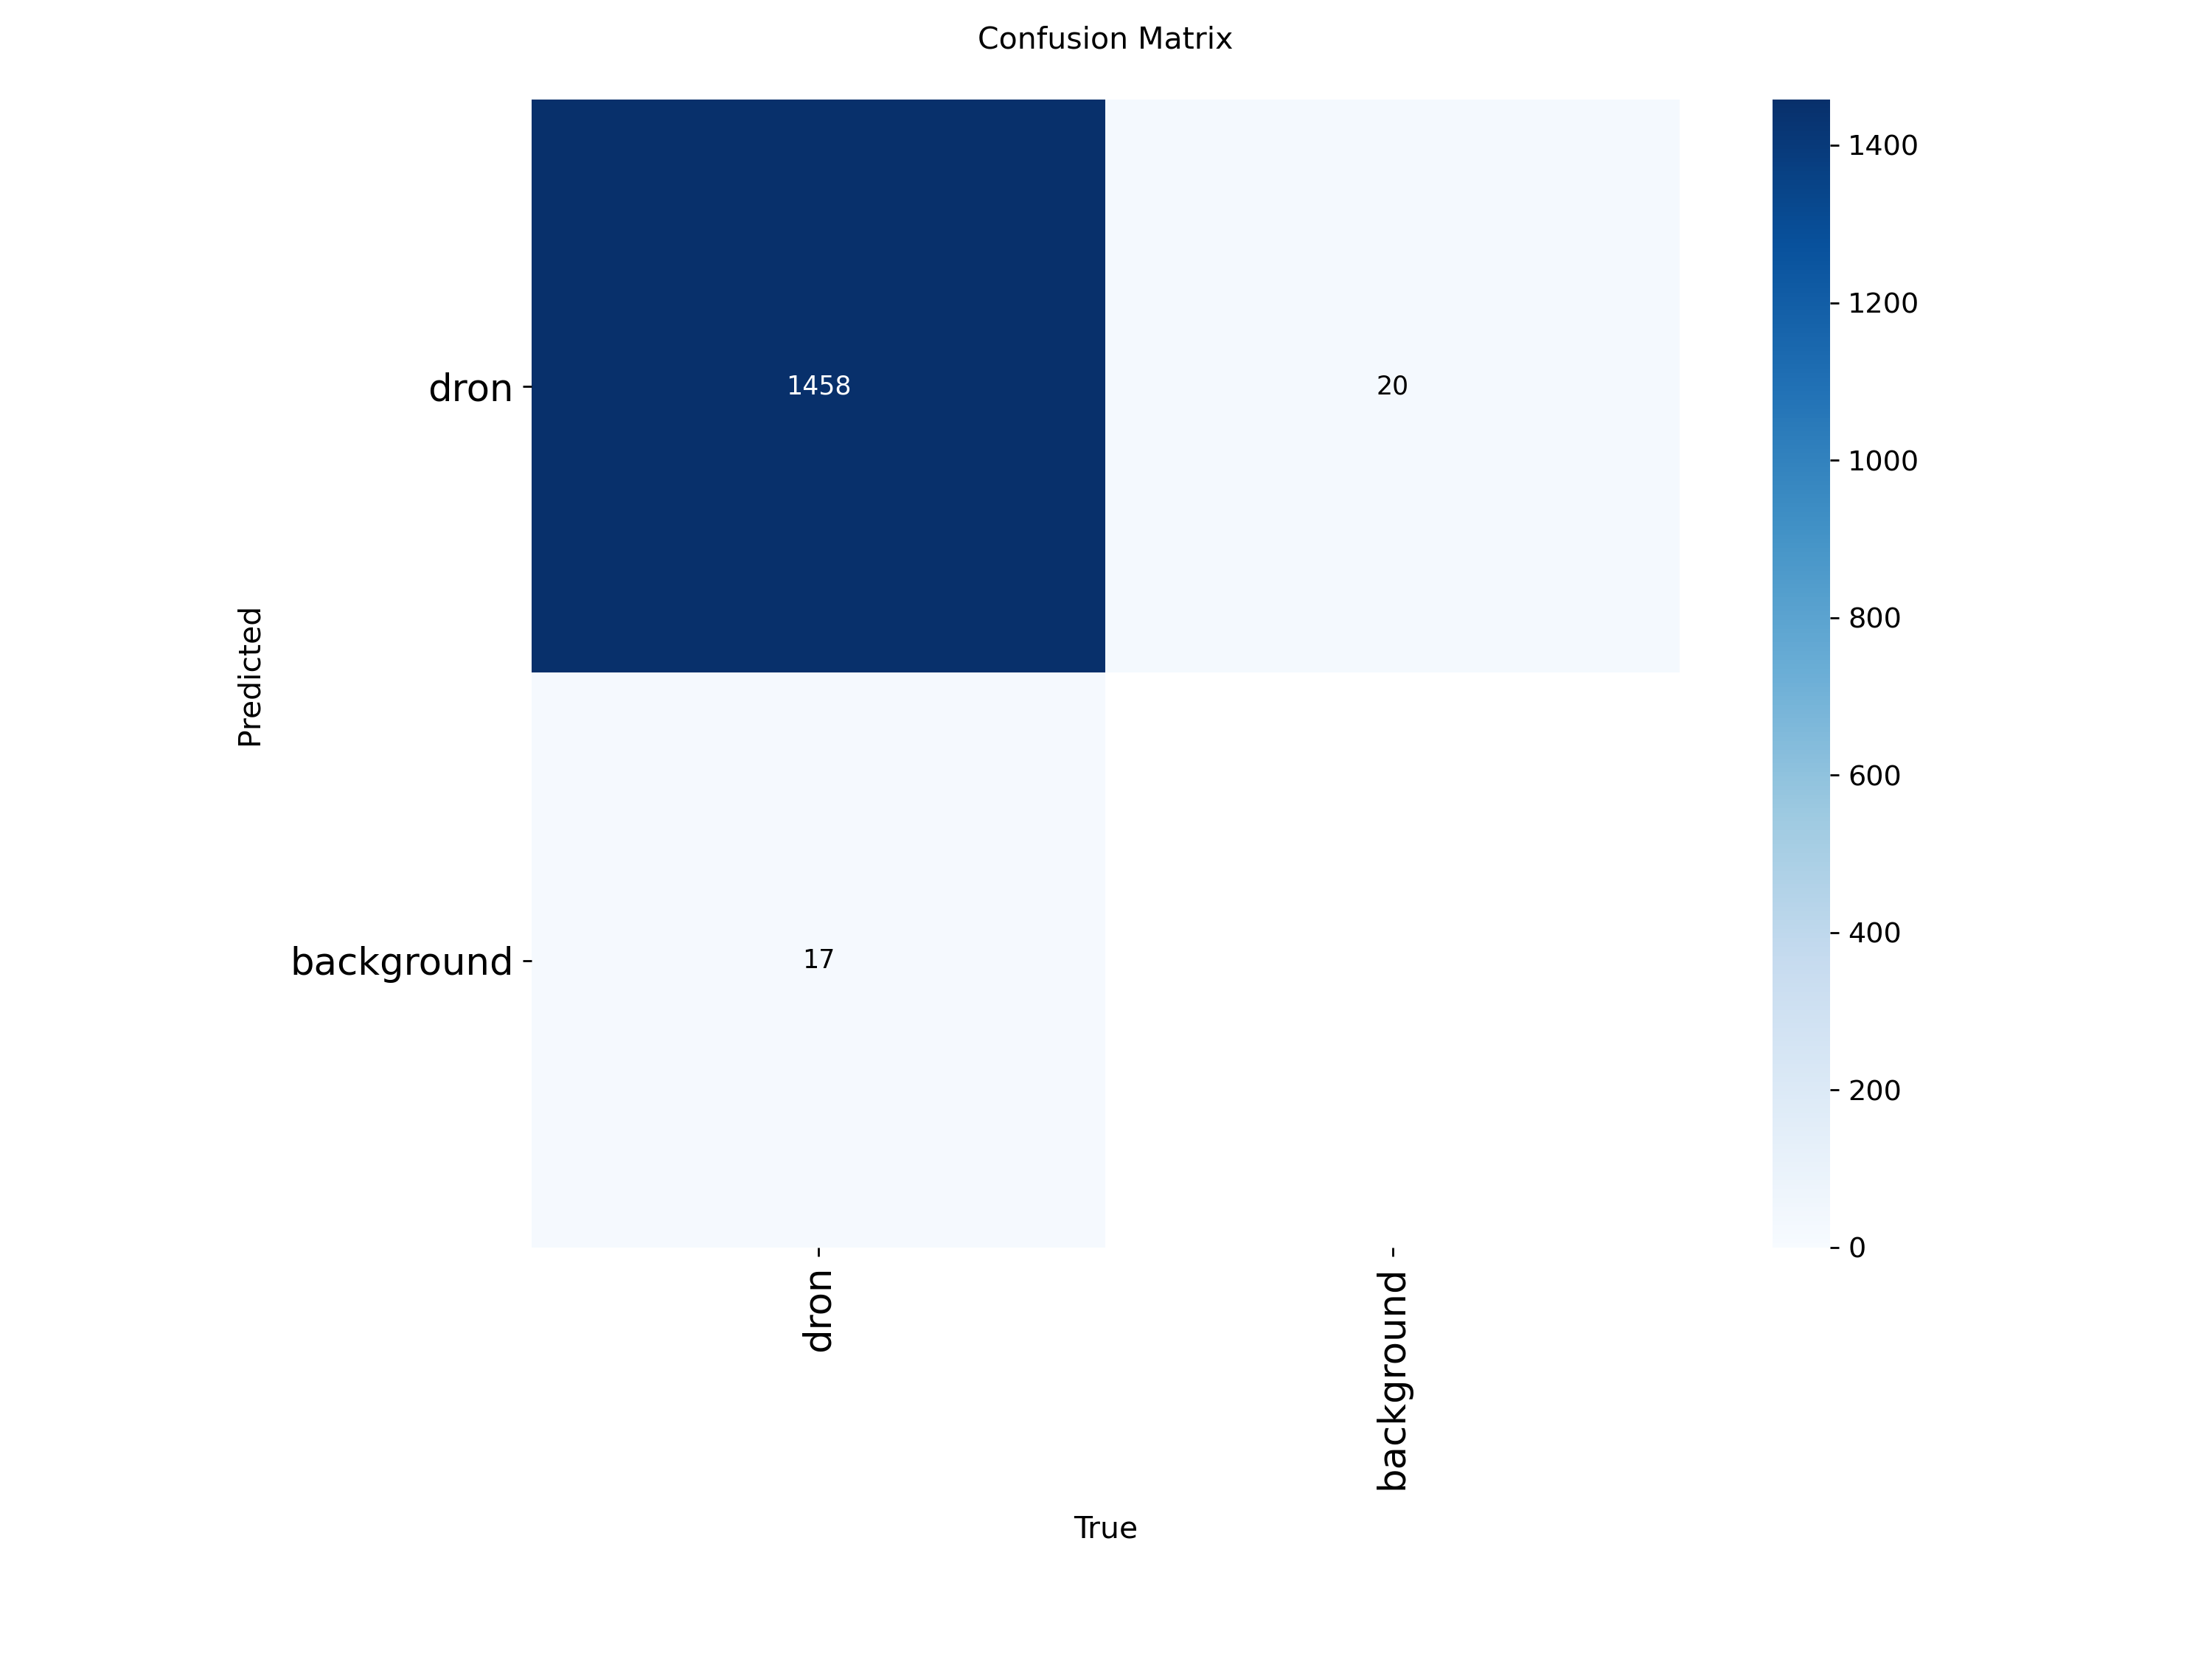
\includegraphics[width=1.0\textwidth]{imagenes/confusion_matrix.png}
\caption{Matriz de confusión obtenida tras el entrenamiento de YOLOv8n. Imagen de elaboración propia.}
\label{fig:yolo-confusion-matrix}
\end{figure}

\vspace{0.3cm}

Por último, la Figura \ref{fig:yolo-validation-predictions} muestra ejemplos de predicción sobre imágenes de validación. En estos casos, el detector localiza correctamente el UAV y ajusta la caja delimitadora alrededor del objetivo, incluso cuando cambia su escala o su posición dentro de la imagen. Esta comprobación visual resulta útil porque permite verificar que las métricas numéricas se corresponden con detecciones coherentes desde el punto de vista del sistema de control.

\begin{figure}[H]
\centering
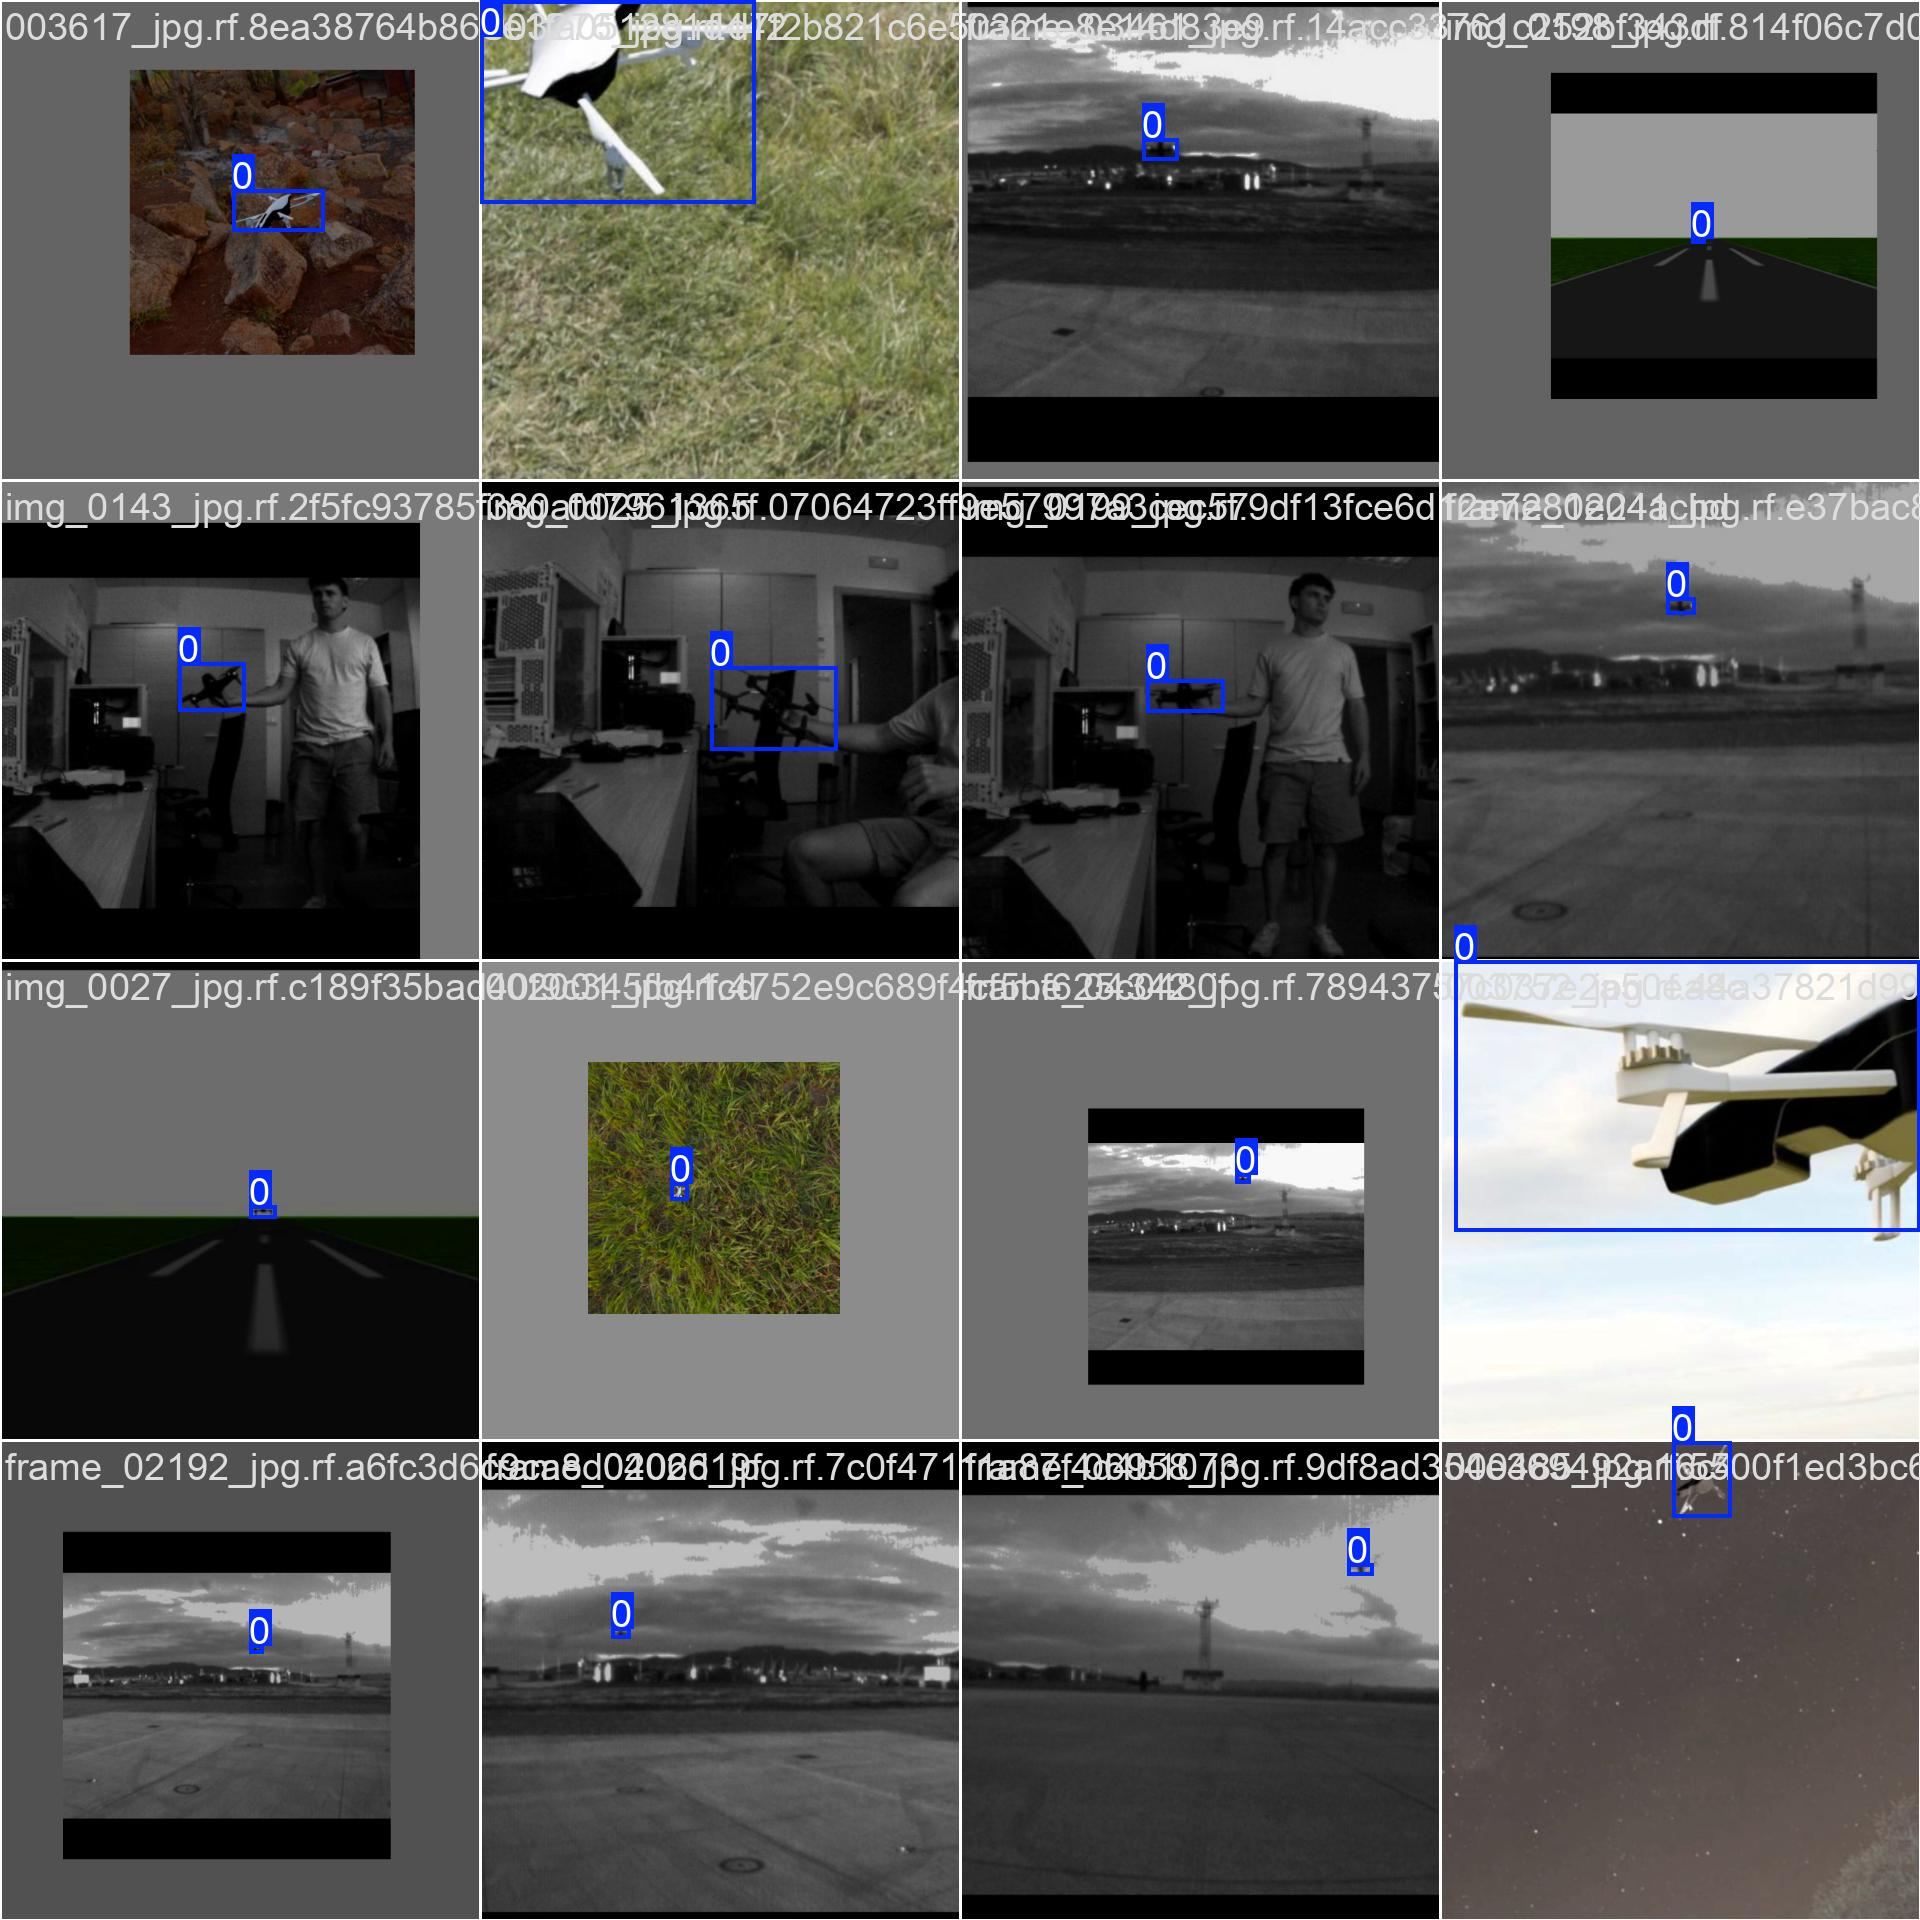
\includegraphics[width=1.0\textwidth]{imagenes/val_batch2_pred.jpg}
\caption{Ejemplos de detección sobre el conjunto de validación tras el entrenamiento. Imagen de elaboración propia.}
\label{fig:yolo-validation-predictions}
\end{figure}

\vspace{0.3cm}

En conjunto, los resultados obtenidos indican que el entrenamiento fue satisfactorio. Las métricas de precisión y \textit{recall} se mantuvieron muy elevadas, el \textit{mAP50} permaneció prácticamente saturado en 0.995 y el \textit{mAP50-95} siguió mejorando de forma progresiva. Además, la reducción simultánea de las pérdidas y la calidad de las predicciones visuales sugieren que el ajuste fino refinó correctamente la localización de las cajas y la clasificación del objetivo sin mostrar signos claros de degradación en validación. Una vez finalizado el entrenamiento, se guardó el mejor modelo obtenido, \texttt{best.pt}, para emplearlo posteriormente en el nodo de percepción visual del sistema.

\subsection{Estimación de la Distancia mediante Ancho y Alto de la Caja}

La estimación de la distancia al UAV objetivo se realiza a partir de la caja delimitadora proporcionada por el sistema de percepción. En esta parte no se vuelve a desarrollar el suavizado temporal, ya que este se describe en el apartado de estimación y filtrado. Únicamente se considera que la caja utilizada para el cálculo ya ha sido estabilizada previamente, de forma que sus coordenadas, su anchura y su altura presentan menos variaciones entre fotogramas.

\vspace{0.3cm}

El proceso implementado parte de las coordenadas de la caja una vez suavizadas. Después de estabilizar las cuatro coordenadas de la detección, se calcula la anchura y la altura aparentes del UAV objetivo en la imagen:

\begin{equation}
\bar{w}_k = \bar{x}_{2,k} - \bar{x}_{1,k}, \quad
\bar{h}_k = \bar{y}_{2,k} - \bar{y}_{1,k}
\end{equation}

\vspace{0.3cm}

Con estos dos valores se calculan dos estimaciones independientes de la distancia. La primera utiliza la anchura real aproximada del UAV y la focal horizontal de la cámara, mientras que la segunda emplea la altura real aproximada y la focal vertical:

\begin{equation}
D_W = \frac{f_x \cdot W_{real}}{\bar{w}_k}, \quad
D_H = \frac{f_y \cdot H_{real}}{\bar{h}_k}
\end{equation}

\vspace{0.3cm}

En estas expresiones, $f_x$ y $f_y$ representan las focales de la cámara en píxeles, y $W_{real}$ y $H_{real}$ corresponden a las dimensiones reales aproximadas del UAV objetivo. La distancia final se obtiene promediando ambas estimaciones:

\begin{equation}
D_{final} = \frac{D_W + D_H}{2}
\end{equation}

\vspace{0.3cm}

Este procedimiento permite aprovechar simultáneamente la información horizontal y vertical de la detección. Si YOLO genera una caja ligeramente más ancha de lo real, pero mantiene una altura coherente, la estimación basada en la altura compensa parcialmente el error. Del mismo modo, si la altura presenta una pequeña variación, la anchura ayuda a estabilizar el resultado. Así, el sistema obtiene una medida de profundidad más robusta que si dependiera de una sola dimensión de la caja.

\vspace{0.3cm}

Finalmente, la distancia calculada se utiliza como entrada del controlador longitudinal, comparándola con una distancia deseada de seguimiento. De esta forma, el dron cazador puede acercarse o alejarse del objetivo manteniendo un margen de seguridad, sin depender únicamente del desplazamiento del centro de la imagen.

\section{Compensación de Actitud y Proyección}

Durante las primeras pruebas se observó que el error visual no dependía únicamente de la posición real del UAV objetivo dentro de la imagen, sino también de la actitud instantánea del dron cazador. Si se tomaba siempre el centro geométrico de la imagen como referencia, cualquier inclinación de la cámara producía un desplazamiento aparente del objetivo. Esto generaba errores falsos que el controlador interpretaba como movimientos reales del objetivo.

\vspace{0.3cm}

El problema aparecía especialmente en dos situaciones. En primer lugar, cuando el dron cazador avanzaba, debía inclinarse para generar movimiento longitudinal. Esta inclinación modificaba la orientación de la cámara y hacía que el objetivo apareciera desplazado verticalmente en la imagen, aunque su posición relativa no hubiese cambiado de forma equivalente. Como consecuencia, el error vertical aumentaba y el controlador de altura podía intentar corregir una desviación que realmente estaba producida por el propio \textit{pitch} del UAV.

\vspace{0.3cm}

En segundo lugar, al realizar giros o movimientos laterales, el dron podía ladearse. Este \textit{roll} rotaba el plano de la imagen y acoplaba parte del error horizontal con el error vertical. Es decir, un desplazamiento producido por la actitud del dron podía aparecer como una variación en el eje vertical de la imagen, generando órdenes de altura innecesarias. Para evitar este comportamiento, se decidió compensar la referencia visual usando la orientación real de la cámara antes de calcular el error.

\vspace{0.3cm}

\begin{center}
\refstepcounter{figure}\label{fig:compensacion-actitud}
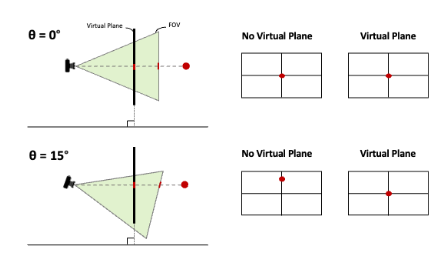
\includegraphics[width=0.78\textwidth]{imagenes/Compensacion.png}\\[0.5ex]
{\small \textbf{Figura \thefigure.} Esquema de compensación de actitud aplicado al plano de imagen. Fuente: ACTA Press \cite{actapressCompensacion}.}
\addcontentsline{lof}{figure}{\protect\numberline{\thefigure}Esquema de compensación de actitud aplicado al plano de imagen}
\end{center}

\vspace{0.3cm}

La Figura \ref{fig:compensacion-actitud} ilustra la idea utilizada para desplazar la referencia de la imagen en función de la actitud de la cámara. En lugar de emplear un centro fijo, se proyecta un rayo compensado que representa el nuevo punto de referencia sobre el plano visual.

\vspace{0.3cm}

La compensación se implementa a partir de la pose del dron cazador en \textit{Gazebo} y de la transformación fija entre el cuerpo del dron y la cámara. En primer lugar, se construye la transformación homogénea del dron en el mundo y se compone con la transformación de la cámara:

\begin{equation}
\mathbf{T}_{w}^{c} = \mathbf{T}_{w}^{d1} \mathbf{T}_{d1}^{c}
\end{equation}

\vspace{0.3cm}

De esta transformación se extrae la matriz de rotación de la cámara y se convierte a ángulos de \textit{roll}, \textit{pitch} y \textit{yaw}:

\begin{equation}
\mathbf{R}_{w}^{c} = \mathbf{T}_{w}^{c}(1{:}3,1{:}3), \quad
(\phi, \theta, \psi) = \mathrm{RPY}(\mathbf{R}_{w}^{c})
\end{equation}

\vspace{0.3cm}

A continuación, se genera una rotación de compensación utilizando únicamente las componentes de \textit{pitch} y \textit{roll}. Siguiendo la convención de ejes empleada en el nodo, esta rotación se construye como:

\begin{equation}
\mathbf{q}_{comp} = \mathbf{q}_{pitch}(\theta) \mathbf{q}_{roll}(\phi)
\end{equation}

\vspace{0.3cm}

Esta rotación se aplica sobre el rayo ideal de la cámara, definido como un vector que apunta hacia delante en el eje óptico:

\begin{equation}
\mathbf{r}_{0} = \left[ \begin{array}{ccc} 0 & 0 & 1 \end{array} \right]^T, \quad
\mathbf{r}_{comp} = \mathbf{R}(\mathbf{q}_{comp})\mathbf{r}_{0}
\end{equation}

\vspace{0.3cm}

El vector resultante representa hacia dónde debería desplazarse el centro de referencia de la imagen cuando la cámara está inclinada. Para obtener ese punto en coordenadas de imagen, el rayo compensado se proyecta mediante el modelo de cámara y los parámetros intrínsecos:

\begin{equation}
\left[ \begin{array}{ccc} u_c & v_c & 1 \end{array} \right]^T \sim
\mathbf{K}\mathbf{r}_{comp}
\end{equation}

\vspace{0.3cm}

En la implementación, esta proyección se realiza con \texttt{cv::projectPoints} y posteriormente se corrige con \texttt{cv::undistortPoints}, empleando la matriz intrínseca \texttt{camera\_matrix} y los coeficientes de distorsión \texttt{dist\_coeffs}. El punto obtenido, $(u_c, v_c)$, sustituye al centro geométrico de la imagen como referencia del controlador. Por ello, el error visual final se calcula como:

\begin{equation}
e_x = \frac{u_c - u_{YOLO}}{W/2}, \quad
e_y = \frac{v_c - v_{YOLO}}{H/2}
\end{equation}

\vspace{0.3cm}

De este modo, el controlador no intenta centrar el objetivo respecto al centro fijo de la imagen, sino respecto al centro compensado según la inclinación real de la cámara. Esto reduce los errores verticales artificiales producidos por el avance del dron y por los ladeos durante maniobras laterales.

\vspace{0.3cm}

No obstante, la compensación no se aplicó a todas las componentes de la orientación. En particular, no se incluyó el \textit{yaw} dentro de la rotación compensada, ya que esto podía producir un efecto no deseado similar a una brújula: el punto de referencia de la imagen quedaría condicionado por el rumbo absoluto del dron y no solo por la inclinación de la cámara. En ese caso, durante los giros, el sistema podría desplazar artificialmente la referencia visual y generar correcciones que no corresponden al centrado real del objetivo. Por este motivo, la compensación se limitó a las inclinaciones que afectan directamente al plano de imagen, dejando que el control de \textit{yaw} se encargue de corregir el error horizontal de seguimiento.

\vspace{0.3cm}

\section{Componente de Control}

Los valores de los controladores PID se obtuvieron mediante un proceso de ajuste empírico iterativo en simulación. En primer lugar, se fijaron ganancias proporcionales bajas para comprobar el sentido de actuación de cada eje y evitar respuestas bruscas. Después se aumentó progresivamente la ganancia proporcional hasta obtener una corrección rápida del error sin provocar oscilaciones sostenidas. A continuación, se introdujo la componente derivativa para amortiguar los cambios rápidos de la señal de error y reducir el sobreimpulso. Finalmente, se añadió una componente integral pequeña para compensar errores residuales en régimen permanente, evitando que la acumulación integral generase órdenes excesivas.

\vspace{0.3cm}

Durante este ajuste también se limitaron las salidas de cada controlador. De esta forma, aunque el error visual o el error de distancia aumenten de forma puntual, las consignas enviadas al autopiloto permanecen dentro de valores admisibles para la simulación. La ley general utilizada para cada controlador se expresa como:

\begin{equation}
u(t) = K_p e(t) + K_i \int_0^t e(\tau)\,d\tau + K_d \frac{de(t)}{dt}
\end{equation}

\vspace{0.3cm}

Posteriormente, la señal calculada se satura para limitar la velocidad angular o lineal enviada a \textit{MAVROS}:

\begin{equation}
u_{sat}(t) = \mathrm{sat}_{[-u_{max},u_{max}]}\left(u(t)\right)
\end{equation}

\vspace{0.3cm}

En el caso del control horizontal, el error de entrada es el desplazamiento visual compensado en el eje horizontal, denominado \texttt{ex\_virtual}. Este error alimenta el PID de \textit{yaw}, cuya salida es la velocidad angular \texttt{w\_yaw}:

\begin{equation}
\omega_{yaw} = \mathrm{sat}_{[-10,10]}\left(
2.365625\,e_{x,virtual}(t)
+ 0.06 \int_0^t e_{x,virtual}(\tau)\,d\tau
+ 0.320\,\frac{de_{x,virtual}(t)}{dt}
\right)
\end{equation}

\vspace{0.3cm}

Para el control vertical se emplea el error \texttt{ey\_virtual}. Este controlador genera la velocidad vertical \texttt{v\_y}, responsable de corregir la posición aparente del objetivo en altura:

\begin{equation}
v_y = \mathrm{sat}_{[-5,5]}\left(
2.15\,e_{y,virtual}(t)
+ 0.0 \int_0^t e_{y,virtual}(\tau)\,d\tau
+ 0.205\,\frac{de_{y,virtual}(t)}{dt}
\right)
\end{equation}

\vspace{0.3cm}

Finalmente, el control longitudinal utiliza el error de distancia estimada, \texttt{e\_dist}, calculado a partir de la diferencia entre la distancia estimada al UAV objetivo y la distancia de referencia. Su salida es la velocidad frontal \texttt{v\_x}:

\begin{equation}
v_x = \mathrm{sat}_{[-5,5]}\left(
0.8\,e_{dist}(t)
+ 0.0 \int_0^t e_{dist}(\tau)\,d\tau
+ 0.35\,\frac{de_{dist}(t)}{dt}
\right)
\end{equation}

\vspace{0.3cm}

La Tabla \ref{tab:pid-control} resume las ganancias y los límites finalmente utilizados en los tres controladores implementados.

\begin{table}[htpb]
\centering
\small
\resizebox{\textwidth}{!}{%
\begin{tabular}{|l|c|c|c|c|c|c|}
\hline
\textbf{Controlador} & \textbf{Entrada} & \textbf{Salida} & \textbf{$K_p$} & \textbf{$K_i$} & \textbf{$K_d$} & \textbf{Límite de salida} \\
\hline
PID de \textit{yaw} & \texttt{ex\_virtual} & \texttt{w\_yaw} & 2.365625 & 0.06 & 0.320 & $\pm 10.0$ rad/s \\
\hline
PID de altura & \texttt{ey\_virtual} & \texttt{v\_y} & 2.15 & 0.0 & 0.205 & $\pm 5.0$ m/s \\
\hline
PID de distancia & \texttt{e\_dist} & \texttt{v\_x} & 0.8 & 0.0 & 0.35 & $\pm 5.0$ m/s \\
\hline
\end{tabular}%
}
\caption{Parámetros finales de los controladores PID utilizados para el seguimiento visual.}
\label{tab:pid-control}
\end{table}
